%%%%%%%%%%%%%%%%%%%%%%%%%%%%%%%%%%%%%%%%%
% Article EcoFoG
% Version 2.1 (23/10/2017)
%
% adapté de :
% Stylish Article
% LaTeX Template
% Version 1.0 (31/1/13)
%
% This template has been downloaded from:
% http://www.LaTeXTemplates.com
%
% Original author:
% Mathias Legrand (legrand.mathias@gmail.com)
%
% License:
% CC BY-NC-SA 3.0 (http://creativecommons.org/licenses/by-nc-sa/3.0/)
%
%%%%%%%%%%%%%%%%%%%%%%%%%%%%%%%%%%%%%%%%%


%----------------------------------------------------------------------------------------
%	PACKAGES AND OTHER DOCUMENT CONFIGURATIONS
%----------------------------------------------------------------------------------------

\documentclass[fleqn,10pt]{ArtEcoFoG} % Document font size and equations flushed left

\setcounter{tocdepth}{3} % Show only three levels in the table of contents section: sections, subsections and subsubsections


% Pandoc environments
\usepackage{framed}
\usepackage{fancyvrb}
\providecommand{\tightlist}{%
  \setlength{\itemsep}{0pt}\setlength{\parskip}{0pt}}
\newcommand{\VerbBar}{|}
\newcommand{\VERB}{\Verb[commandchars=\\\{\}]}
\DefineVerbatimEnvironment{Highlighting}{Verbatim}{commandchars=\\\{\}, fontsize=\scriptsize} % Code R
\definecolor{shadecolor}{RGB}{248,248,248}
\newenvironment{Shaded}{\begin{snugshade}}{\end{snugshade}}
\newcommand{\KeywordTok}[1]{\textcolor[rgb]{0.13,0.29,0.53}{\textbf{{#1}}}}
\newcommand{\DataTypeTok}[1]{\textcolor[rgb]{0.13,0.29,0.53}{{#1}}}
\newcommand{\DecValTok}[1]{\textcolor[rgb]{0.00,0.00,0.81}{{#1}}}
\newcommand{\BaseNTok}[1]{\textcolor[rgb]{0.00,0.00,0.81}{{#1}}}
\newcommand{\FloatTok}[1]{\textcolor[rgb]{0.00,0.00,0.81}{{#1}}}
\newcommand{\ConstantTok}[1]{\textcolor[rgb]{0.00,0.00,0.00}{{#1}}}
\newcommand{\CharTok}[1]{\textcolor[rgb]{0.31,0.60,0.02}{{#1}}}
\newcommand{\SpecialCharTok}[1]{\textcolor[rgb]{0.00,0.00,0.00}{{#1}}}
\newcommand{\StringTok}[1]{\textcolor[rgb]{0.31,0.60,0.02}{{#1}}}
\newcommand{\VerbatimStringTok}[1]{\textcolor[rgb]{0.31,0.60,0.02}{{#1}}}
\newcommand{\SpecialStringTok}[1]{\textcolor[rgb]{0.31,0.60,0.02}{{#1}}}
\newcommand{\ImportTok}[1]{{#1}}
\newcommand{\CommentTok}[1]{\textcolor[rgb]{0.56,0.35,0.01}{\textit{{#1}}}}
\newcommand{\DocumentationTok}[1]{\textcolor[rgb]{0.56,0.35,0.01}{\textbf{\textit{{#1}}}}}
\newcommand{\AnnotationTok}[1]{\textcolor[rgb]{0.56,0.35,0.01}{\textbf{\textit{{#1}}}}}
\newcommand{\CommentVarTok}[1]{\textcolor[rgb]{0.56,0.35,0.01}{\textbf{\textit{{#1}}}}}
\newcommand{\OtherTok}[1]{\textcolor[rgb]{0.56,0.35,0.01}{{#1}}}
\newcommand{\FunctionTok}[1]{\textcolor[rgb]{0.00,0.00,0.00}{{#1}}}
\newcommand{\VariableTok}[1]{\textcolor[rgb]{0.00,0.00,0.00}{{#1}}}
\newcommand{\ControlFlowTok}[1]{\textcolor[rgb]{0.13,0.29,0.53}{\textbf{{#1}}}}
\newcommand{\OperatorTok}[1]{\textcolor[rgb]{0.81,0.36,0.00}{\textbf{{#1}}}}
\newcommand{\BuiltInTok}[1]{{#1}}
\newcommand{\ExtensionTok}[1]{{#1}}
\newcommand{\PreprocessorTok}[1]{\textcolor[rgb]{0.56,0.35,0.01}{\textit{{#1}}}}
\newcommand{\AttributeTok}[1]{\textcolor[rgb]{0.77,0.63,0.00}{{#1}}}
\newcommand{\RegionMarkerTok}[1]{{#1}}
\newcommand{\InformationTok}[1]{\textcolor[rgb]{0.56,0.35,0.01}{\textbf{\textit{{#1}}}}}
\newcommand{\WarningTok}[1]{\textcolor[rgb]{0.56,0.35,0.01}{\textbf{\textit{{#1}}}}}
\newcommand{\AlertTok}[1]{\textcolor[rgb]{0.94,0.16,0.16}{{#1}}}
\newcommand{\ErrorTok}[1]{\textcolor[rgb]{0.64,0.00,0.00}{\textbf{{#1}}}}
\newcommand{\NormalTok}[1]{{#1}}
\usepackage{longtable,booktabs}
\usepackage{caption}
% These lines are needed to make table captions work with longtable:
\makeatletter
\def\fnum@table{\tablename~\thetable}
\makeatother
% longtable 2 columns
% https://tex.stackexchange.com/questions/161431/how-to-solve-longtable-is-not-in-1-column-mode-error
\makeatletter
\let\oldlt\longtable
\let\endoldlt\endlongtable
\def\longtable{\@ifnextchar[\longtable@i \longtable@ii}
\def\longtable@i[#1]{\begin{figure}[t]
\onecolumn
\begin{minipage}{0.5\textwidth}\scriptsize
\oldlt[#1]
}
\def\longtable@ii{\begin{figure}[t]
\onecolumn
\begin{minipage}{0.5\textwidth}\scriptsize
\oldlt
}
\def\endlongtable{\endoldlt
\end{minipage}
\twocolumn
\end{figure}}
\makeatother

\usepackage{graphicx,grffile}
\makeatletter
\def\maxwidth{\ifdim\Gin@nat@width>\linewidth\linewidth\else\Gin@nat@width\fi}
\def\maxheight{\ifdim\Gin@nat@height>\textheight0.8\textheight\else\Gin@nat@height\fi}
\makeatother
% Scale images if necessary, so that they will not overflow the page
% margins by default, and it is still possible to overwrite the defaults
% using explicit options in \includegraphics[width, height, ...]{}
\setkeys{Gin}{width=\maxwidth,height=\maxheight,keepaspectratio}

% User-adder preamble
\usepackage{amsmath}

%----------------------------------------------------------------------------------------
%	ARTICLE INFORMATION
%----------------------------------------------------------------------------------------

\JournalInfo{~} % Journal information
\Archive{~} % Additional notes (e.g. copyright, DOI, review/research article)

\PaperTitle{Comparing tree diversity between two forest plots, BCI and Paracou} % Article title

\Authors{
Ilke Geladi\textsuperscript{1*}
} % Authors
\affiliation{
\textsuperscript{1}UMR EcoFoG, AgroParistech, CNRS, Cirad, INRA, Université de Guyane.\\ \hspace{1em} Campus Agronomique, 97310 Kourou, France.
}
\affiliation{*\textbf{Contact}: ilke.geladi@ecofog.gf, http://www.ecofog.gf/spip.php?article47} % Corresponding author

\Keywords{Diversity, BCI, Paracou, Diversity Profiles, Hill numbers} % Keywords - if you don't want any simply remove all the text between the curly brackets
\newcommand{\keywordname}{Keywords} % Defines the keywords heading name

%----------------------------------------------------------------------------------------
%	ABSTRACT
%----------------------------------------------------------------------------------------

\Abstract{
BCI is one of the best-studied forest plots on earth, however we must
consider the value of other similar forest plots such as Paracou in
French Guiana. Here, we compare the diversity between the two through
diversity profiles and rarefication of the data. It was found that
Paracou is more diverse than BCI. An increased diversity in a forest
plot holds potential for novel and unique studies that BCI does not
offer.
}

%----------------------------------------------------------------------------------------

\begin{document}

\selectlanguage{english}

\flushbottom % Makes all text pages the same height

\maketitle % Print the title and abstract box

\tableofcontents % Print the contents section

\thispagestyle{empty} % Removes page numbering from the first page

%----------------------------------------------------------------------------------------
%	ARTICLE CONTENTS
%----------------------------------------------------------------------------------------


\section{Introduction}\label{introduction}

Tropical rainforests are the most biodiverse ecosystems in the world,
housing two to three thirds of the species in the world
\citep{Laurance2007c, Noss1999, Bierregaard1992}. Reliable information
on the status and condition in each forest studied, including the
diversity of trees, is crucial to expanding our knowledge in fields such
as forest dynamics, community ecology, and biotic interactions to ensure
the best possible management and conservation strategies
\citep{Condit1995, Noss1999}. However, to collect such knowledge,
long-term studies are necessary as they provide a more wholistic view
through continuous monitoring and data on patterns and rates of change
in forest ecosystems \citep{comiskey1998forest}. Permanent forest plots
are widely used for these sorts of studies
\citep{comiskey1998forest, Condit1995}, and many have been established
in various ecosystems worldwide \citep{Condit2014}.

In the tropics, arguably the most famous long-term forest plot is Barro
Colorado Island (BCI), a 1500-ha island in Panama
\citep{leigh1999tropical}. Scientists have been conducting studies at
BCI since 1916 and it has since become one of the best studied areas of
tropical rainforest in the world \citep{leigh1999tropical}. Despite
this, BCI is not a very diverse or pristine habitat
\citep{leigh1999tropical}, and there are many advantages to conducting
studies at other less-famous forest plots, such as Paracou in French
Guiana \citep{Gourlet-Fleury2004}. Offering more than 100 hectares of
plots, Paracou was established in 1982 and has also been home to many
studies on forest functioning and forestry research programs
\citep{Charles-Dominique2001, Gourlet-Fleury2004}.

In this study we will compare the neutral forest diversity, focusing
solely on trees, of BCI and Paracou. With Paracou being connected to
mainland South America thus having higher colonization rates compared to
BCI which is an island \citep{BRV:BRV510}, we hypothesize that Paracou
is more diverse than BCI. Habitats with increased diversity, such as
Paracou, might increase potential research questions and provide
different opportunities to further increase our knowledge of tropical
rainforests compared to BCI.

\section{Materials and Methods}\label{materials-and-methods}

\subsection{Study Sites}\label{study-sites}

\subsubsection{BCI}\label{bci}

For the first study site, we used tree diversity data from Barro
Colorado Island (BCI) \citep{croat1978flora}, which can be found in the
``vegan'' package\citep{oksanen2010vegan}. BCI became an island with the
damming of the Chagres River in Panama between 1911 and 1914 and was
subsequently named a biological reserve in 1923, which is currently
supervised by the Smithsonian Tropical Research Institute (STRI)
\citep{croat1978flora, leigh1999tropical}. It is a 1,560-hectare island
that welcomes hundreds scientists from around the world each year
\citep{croat1978flora}.

\subsubsection{Paracou}\label{paracou}

For the second study site, we used tree diversity data from Paracou
\citep{Degen2006}, which can be found in the ``entropart'' package
\citep{Marcon2014c}.

Paracou is located in French Guiana, and has been used since 1982 for
basic ecological research on lowland rainforest
\citep{Gourlet-Fleury2004}. The site is more than 1000 hectares large
and trees have been fully mapped as Paracou was used as an experimental
design to study the impact of disturbances on forest stands and tree
populations \citep{Gourlet-Fleury2004}.

\subsection{Diversity Comparison}\label{diversity-comparison}

To compare the two study sites, we first compared their asymptotic
diversity profiles. To do this we used the ``CommunityProfile'' function
in the ``entropart'' package \citep{Marcon2014c} to create the diveristy
profile for both sites followed by the ``CEnvelope'' function
\citep{Marcon2014c} to add the BCI diversity profile to that of Paracou.
Hill Numbers were then calculated when q is equal to 0, 1 and 2 using
the ``Diversity'' function \citep{Marcon2014c}.

Next, we rarified the data to the same coverage as an alternative method
to compare the two communities whilst accounting for the difference in
study site size. Through this method, we simulate the decrease in the
size of the large community, in this case Paracou, to reduce it to the
size of the small community, BCI \citep{marcon2017}. In the process, we
loose some data, however it is better to loose some data than have a lot
of uncertainty, which is the case when estimating the asymptotic
diversity. To do so, we used the function ``estimateD''" of the package
iNEXT \citep{hsieh2016inext}, and compared the data for values of
diveristy of q=0, 1 and 2, rarified to the same coverage of 80\%. All
above analyses and calculations were performed in R \citep{R}.

\section{Results}\label{results}

\begin{figure}
\centering
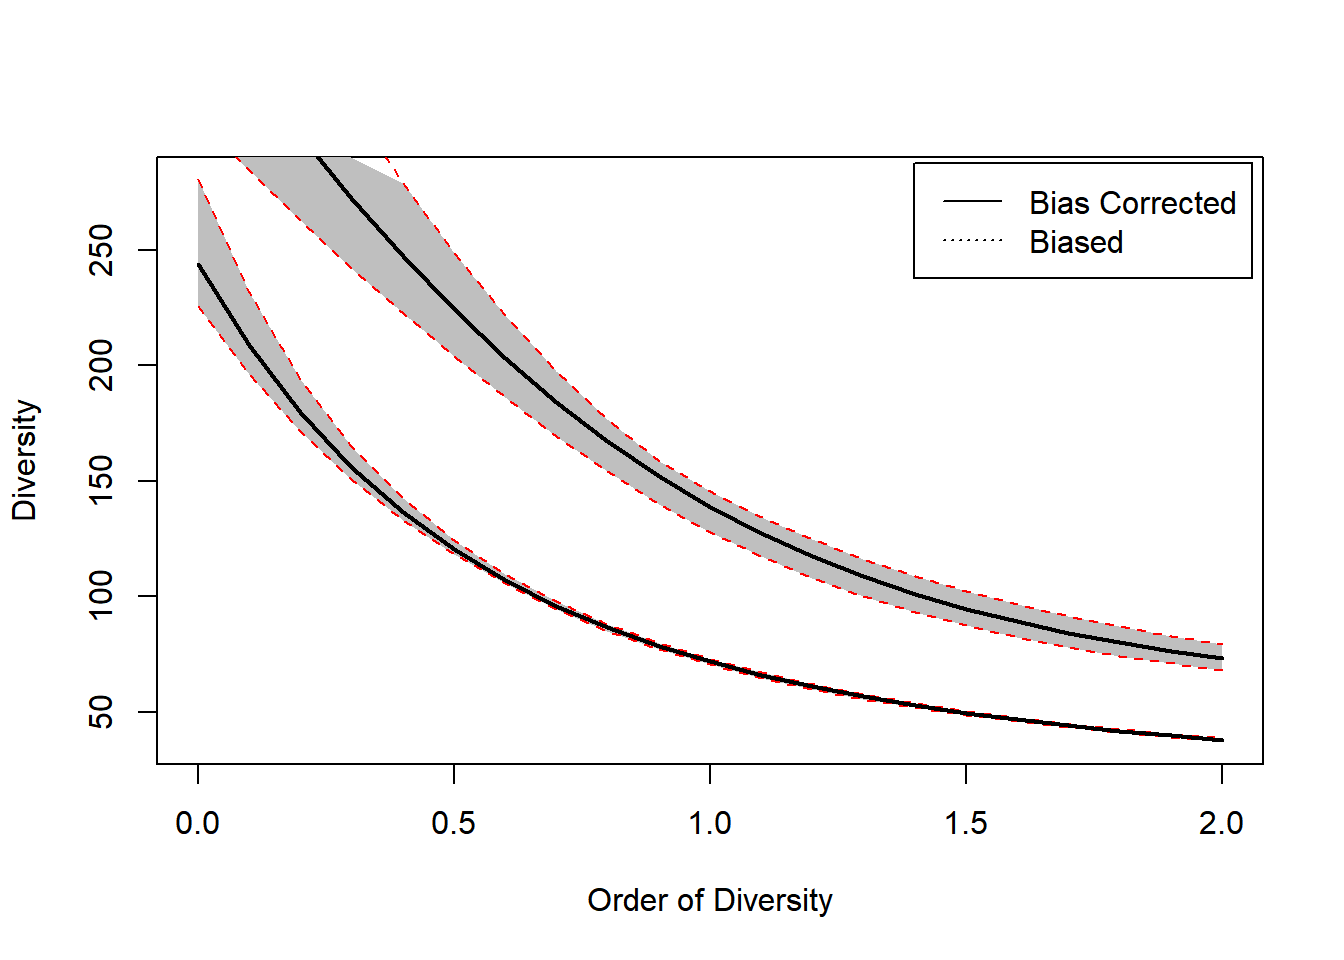
\includegraphics{CoursEric_files/figure-latex/dp-1.pdf}
\caption{\label{fig:dp}Diversity Profiles for Paracou (top line) and BCI
(bottom line). Confidence intervals are obtained by bootstrap from 1000
simulations.}
\end{figure}

Asymptotic diversity profiles reveal Paracou to be more diverse than BCI
(See \ref{fig:dp}). As can be seen in Figure \ref{fig:dp}, the Paracou
diversity profile curve is above the BCI curve for all values of q. This
is confirmed by calculating the Hill numbers for both BCI and Paracou.
It was found that Paracou was more diverse at all order's of q where for
when q equals 0, 1 and 2, the corresponding Hill numbers for Paracou
were 315, 133 and 73, and for BCI were 239, 72 and 38.

BCI and Paracou data rarified to the same coverage (80\%) also reveals
Paracou to have a greater diversity at order of diversities 0, 1 and 2
compared to BCI. Species richness (q=0) of Paracou (S=136) is almost
double that of BCI (S=69). The exponential of Shannon's entropy index
(q=1) of Paracou is 89, whereas that of BCI is only 47. Finally, when
q=2 (the inverse of Simpson's concentration index), diversity of Paracou
is once again almost double that of BCI where Paracou's is at 61 and
BCI's at 31.

\section{Discussion}\label{discussion}

Diversity Profiles show that tree diversity is more neutrally diverse in
Paracou than in BCI, as the Paracou curve is above the the BCI curve. It
can further be said that BCI and Paracou are separable as the
communities diversity profiles do not intersect \citep{marcon2017}.
There has been much debate as to which diversity indices to use as there
exist many. However, diversity profiles play an important role in
converging these indices by portraying them graphically as the value of
diversity is plotted in function to the order q, which represent
different indices \citep{Tothmeresz1995, marcon2017}. The raw result of
the Hill numbers calculated support the above conclusion that Paracou is
more diverse than BCI. Hill numbers provide many advantages over other
frequent used measures of diversity, such as species richness, through
incorporating both relative abundance and species richness, amongst
other reasons \citep{Chao2014}. Overall, diversity profiles and Hill
numbers, which are two more reliable methods of calculating diversity,
reveal that Paracou has a higher tree diversity than BCI.

Rarefaction results support the conclusions from the diversity profiles,
taking it a step further and revealing the tree diversity in Paracou is
almost double that of BCI (when q=0 and q=2). Rarefaction of the data is
important as it standardizes the data on the basis of sample size or
sample completeness thus facilitating and providing a more accurate view
of the comparison between both forest plots \citep{Chao2014}. Having
both diversity profiles and rarefied data support that Paracou is more
diverse than BCI, we can be certain of this conclusion.

A logical explanation as to why Paracou is more diverse than BCI is
related to island biogeography theory where it predicts that with
increased colonization, there is more diversity \citep{BRV:BRV510}.
Seeing as Paracou is on continental land, it is very connected to other
communities where colonization is facilitated compared to BCI which is
an island. Furthermore, island populations have a much higher risk of
extinction than mainland populations \citep{Frankham1997}. However, it
must also be recognized that often islands have higher speciation rates
and thus more endemic species, being valuable in a different way than
mainland ecosystems, which is not taken into account by these
calculations \citep{Kier9322}.

Studying diversity is very important in ecological theory and practice
\citep{Tothmeresz1995}. Diversity indices are often used as indicators
of the `well-being' of an ecosystem and are thus implicated in
conservation management and environmental monitoring
\citep{Tothmeresz1995, Chao2014}.

In conclusion, Paracou is more diverse than BCI. Studying diversity is
important as it informs us about the state of the ecosystem, and has
implications in management strategies. Eventhough BCI has the advantage
of being very well-studied and potentially having more endemic species
than Paracou, Paracou has a higher diversity than BCI which can provide
very interesting research opportunities compared to BCI.

%----------------------------------------------------------------------------------------
%	REFERENCE LIST
%----------------------------------------------------------------------------------------

\bibliographystyle{mee}
\bibliography{library}

%----------------------------------------------------------------------------------------

\end{document}
